% Provenance (never printed): see sources/outline_sources.md (Year 3: refraction and
% reflection seismic methods; CMP acquisition, NMO, stacking, Dix; migration in
% principle; seismic stratigraphy). Brief: sources/book5/BRIEFS.md, ch. 2. Curves from
% figdata/bachelor-3/seismic_model.py, refraction_dip.py, synthetic_seismogram.py,
% cmp_nmo.py (the Varden column, region.py); exercise and problem values in the
% Book 5 scratch calculator calc/ch02.py.
\chapter{Sismologia de exploração}\label{ch:b3:exploration-seismology}

Um navio de levantamento navega lentamente em linha reta no mar, rebocando um conjunto de
canhões de ar a poucos metros abaixo da superfície e, atrás dele, cabos com vários
quilômetros de comprimento, equipados com hidrofones. Em um levantamento descrito ao
órgão regulador, o conjunto continha \num{5240} polegadas cúbicas de ar comprimido, disparado a cada
\qty{8}{s} a partir de \qty{12}{m} abaixo da superfície, e os cabos rebocados de azimute estreito
atrás de navios desse tipo registram afastamentos de 8 a \qty{10}{km}.
% ledger: noaa5:wg-survey
Cada tiro envia um pulso sonoro para o fundo do mar, e cada interface de rochas
abaixo devolve um eco fraco. Semanas de processamento depois, um geólogo percorre
uma seção transversal em que canais fluviais soterrados, blocos de falha inclinados e
o preenchimento em \omterm{def:b3:exploration-seismology:terminations}{onlap} de uma bacia antiga aparecem como se o terreno tivesse sido cortado ao meio.
A sismologia em escala terrestre do capítulo anterior usou as ondas de
terremotos; a sismologia de exploração produz as suas próprias, com fontes cujo instante e
local são conhecidos com exatidão, e as registra em milhares de canais. Este
capítulo acompanha os ecos desde o tiro até a seção: levantamentos de refração,
a reflexão de uma ondaleta por uma coluna estratificada, o método do \omterm{def:b3:exploration-seismology:cmp}{ponto médio comum}
que transforma ecos repetidos em velocidades e em uma imagem limpa, a migração, que
recoloca os refletores em suas posições corretas, e a leitura da seção como
estratigrafia.

\begin{recall}
Em uma fronteira entre dois meios de impedâncias acústicas $Z_1 = \rho_1v_1$ e
$Z_2 = \rho_2v_2$, uma onda plana em incidência normal é refletida com o
coeficiente de amplitude $R = (Z_2 - Z_1)/(Z_2 + Z_1)$ (o volume do segundo ano dos livros de física
volume, sobre ondas em interfaces). A onda de cabeça, o tempo de intercepto e a
distância de cruzamento de um perfil de refração sobre camadas planas foram vistos no
volume do primeiro ano, no capítulo sobre a Terra estratificada; os perfis de sondagem no livro~2
(11º ano). A convolução $(f*g)(t) = \int f(\tau)g(t - \tau)\,\mathrm d\tau$
e a transformada de Fourier são dos livros de matemática. O \omterm{def:b3:seismology-imaging:ray-parameter}{parâmetro do raio} e o
\omterm{def:b3:seismology-imaging:inverse}{problema inverso} linear são os do \cref{ch:b3:seismology-imaging}.
\end{recall}

\section{Levantamentos de refração}

\begin{definition}[Levantamentos de refração e de reflexão sísmica]\label{def:b3:exploration-seismology:surveys}
Um \emph{levantamento de refração sísmica}\index{levantamento de refração sísmica} registra, ao longo
de uma linha de receptores, as primeiras chegadas de uma fonte controlada, e usa as
ondas de cabeça que se propagam pelo topo de camadas mais rápidas para determinar suas velocidades e
profundidades. Um \emph{levantamento de reflexão sísmica}\index{levantamento de reflexão sísmica}
registra o trem de ondas completo, com afastamentos em geral menores que as profundidades de
interesse, e usa as ondas refletidas em incidência quase normal pelas
interfaces para obter a imagem do acamamento.
\end{definition}

Sobre camadas planas, uma onda de cabeça chega em $t = x/v_2 + t_i$, uma reta
cujo coeficiente angular fornece a velocidade $v_2$ do refrator e cujo intercepto $t_i$
fornece sua profundidade. Um refrator inclinado inclina a reta: a onda de cabeça disparada
a favor do mergulho chega cada vez mais tarde, à medida que o refrator se aprofunda, e parece lenta;
disparada contra o mergulho parece rápida. Disparando nos dois sentidos ao longo da mesma linha, um perfil reverso
separa a velocidade do mergulho.

\begin{theorem}[Refração em uma interface inclinada]\label{thm:b3:exploration-seismology:dipping}
Uma camada de velocidade $v_1$ sobrepõe um refrator plano de velocidade $v_2 > v_1$ com mergulho
no ângulo $\theta$ ao longo do perfil; $i_c = \arcsin(v_1/v_2)$, e $h$ é a
profundidade perpendicular do refrator sob o tiro. Além da distância crítica,
a onda de cabeça chega em
\begin{align*}
  t &= \frac{x\sin(i_c + \theta)}{v_1} + \frac{2h\cos i_c}{v_1}
  &&\text{disparada a favor do mergulho},\\
  t &= \frac{x\sin(i_c - \theta)}{v_1} + \frac{2h\cos i_c}{v_1}
  &&\text{disparada contra o mergulho}.
\end{align*}
As velocidades aparentes $v_d = v_1/\sin(i_c + \theta)$ e
$v_u = v_1/\sin(i_c - \theta)$ de um perfil reverso fornecem
\[
  i_c = \tfrac12\left[\arcsin\frac{v_1}{v_d} + \arcsin\frac{v_1}{v_u}\right],\qquad
  \theta = \tfrac12\left[\arcsin\frac{v_1}{v_d} - \arcsin\frac{v_1}{v_u}\right],
  \qquad v_2 = \frac{v_1}{\sin i_c} .
\]
\end{theorem}

\begin{proof}
Gira-se o referencial de modo que o refrator fique horizontal; a superfície então mergulha segundo o ângulo
$\theta$, e, disparando a favor do mergulho, a profundidade perpendicular sob um receptor no
afastamento $x$ é $h + x\sin\theta$, cuja projeção sobre o refrator é
$x\cos\theta$. O caminho da onda de cabeça desce com o ângulo crítico $i_c$ até a
normal, percorre o refrator com velocidade $v_2$ e sobe com $i_c$. Seu tempo é
\[
  t = \frac{h}{v_1\cos i_c} + \frac{x\cos\theta - h\tan i_c - (h + x\sin\theta)\tan i_c}{v_2}
  + \frac{h + x\sin\theta}{v_1\cos i_c}.
\]
Com $1/v_2 = \sin i_c/v_1$ e $1/\cos i_c - \sin i_c\tan i_c = \cos i_c$,
os termos em $h$ dão $2h\cos i_c/v_1$ e os em $x$ dão
$x(\sin i_c\cos\theta + \cos i_c\sin\theta)/v_1 = x\sin(i_c + \theta)/v_1$.
Contra o mergulho, $\theta$ muda de sinal. As últimas fórmulas invertem as duas
velocidades aparentes.
\end{proof}

Os dois ramos de um perfil reverso devem dar o mesmo tempo entre os dois
pontos de tiro, qualquer que seja a extremidade disparada: o \emph{tempo recíproco}, uma verificação da
leitura dos tempos. Duas situações invalidam o método. Uma camada mais lenta que a de cima
(uma inversão de velocidade) não refrata onda de cabeça alguma e é invisível: suas rochas são
contadas na camada de cima, e toda profundidade abaixo é superestimada. Uma camada
mais rápida que a de cima, mas fina demais, pode nunca dar uma primeira chegada, pois
a onda de cabeça da camada mais profunda e mais rápida a alcança: uma camada oculta. Um
levantamento de reflexão enxerga ambas.

\begin{omfigure}
\begin{tikzpicture}
\begin{axis}[omrecord, width=0.82\linewidth, height=0.46\linewidth,
  xmin=0, xmax=1200, ymin=0, ymax=660,
  xlabel={posição ao longo do arranjo, a partir do tiro O (\unit{m})},
  ylabel={tempo (\unit{ms})}, legend pos=north west, legend cell align=left,
  legend style={font=\scriptsize}]
\addplot[gray, thick, densely dashed] table[x=x, y=tdir] {figdata/out/bachelor-3-refraction_dip-west.dat};
\addlegendentry{ondas diretas ($v_1$)}
\addplot[blue!70!black, thick] table[x=x, y=thead] {figdata/out/bachelor-3-refraction_dip-west.dat};
\addlegendentry{onda de cabeça de O, disparada contra o mergulho}
\addplot[red!70!black, thick] table[x expr=1200-\thisrow{x}, y=thead] {figdata/out/bachelor-3-refraction_dip-east.dat};
\addlegendentry{onda de cabeça de L, disparada a favor do mergulho}
\addplot[gray, thick, densely dashed, forget plot] table[x expr=1200-\thisrow{x}, y=tdir] {figdata/out/bachelor-3-refraction_dip-east.dat};
\addplot[only marks, mark=*, mark size=1.5pt] coordinates {(1200,486.13) (0,486.13)};
\node[font=\scriptsize, anchor=south east] at (axis cs:1190,530) {tempo recíproco};
\end{axis}
\end{tikzpicture}

\par\smallskip{\small Um perfil de refração reverso no flanco oeste do
anticlinal de Varden (calculado; problema, parte I). O refrator, o topo do
calcário, sobe de O para L com \ang{10.8} sob um espalhamento de \qty{1200}{m}; o
giz e o folhelho acima são agrupados em uma única camada de \qty{2.40}{km.s^{-1}}. A
onda de cabeça disparada de O, a montante do mergulho, aparece rápida (\qty{6.57}{km.s^{-1}}); a disparada
de L, a jusante do mergulho, é lenta (\qty{3.52}{km.s^{-1}}); ambas levam \qty{486.1}{ms} para cruzar
todo o espalhamento. As ondas de cabeça só ultrapassam as ondas diretas perto do
extremo distante: o refrator é profundo para um espalhamento tão curto.}
\label{fig:b3:exploration-seismology:refraction}
\end{omfigure}

\section{Reflexão em incidência normal}

\begin{definition}[Ondaleta sísmica, ondaleta de Ricker]\label{def:b3:exploration-seismology:wavelet}
Uma \emph{ondaleta sísmica}\index{ondaleta sísmica} é o pulso curto, de algumas dezenas
de milissegundos de duração, que a fonte e o sistema de registro enviam através do
solo; cada refletor devolve uma cópia escalonada dela. A \emph{ondaleta de
Ricker}\index{ondaleta de Ricker} de frequência de pico $f$ é o pulso de fase zero
\[
  w(t) = \left(1 - 2\pi^2f^2t^2\right)e^{-\pi^2f^2t^2},
\]
a segunda derivada de uma gaussiana, a menos de sinal e escala: um pico central e
dois lóbulos laterais, com média nula e um espectro de amplitude com máximo em $f$.
\end{definition}

\begin{definition}[Série de refletividade]\label{def:b3:exploration-seismology:synthetic}
A \emph{série de refletividade}\index{série de refletividade} de uma coluna estratificada é
a sequência dos coeficientes de reflexão em incidência normal $r_k$ de suas interfaces,
posicionados em seus tempos verticais de ida e volta $\tau_k = \sum_{i \le k} 2h_i/v_i$:
$r(t) = \sum_k r_k\,\delta(t - \tau_k)$.
\end{definition}

\begin{proposition}[O modelo convolucional]\label{prop:b3:exploration-seismology:synthetic}
Se apenas as reflexões primárias são mantidas (sem múltiplas), em incidência normal, sem
perda por transmissão, atenuação ou espalhamento, e a ondaleta $w$ não
varia com a profundidade, o traço registrado é a convolução da ondaleta com a
\omterm{def:b3:exploration-seismology:synthetic}{série de refletividade}:
\[
  s(t) = \sum_k r_k\,w(t - \tau_k) = (w*r)(t) .
\]
O traço calculado desse modo a partir de um perfil de sondagem de velocidade e densidade é o
\emph{sismograma sintético}\index{sismograma sintético} do perfil.
\end{proposition}

\begin{proof}
Cada interface devolve uma cópia da ondaleta incidente, escalonada por seu coeficiente
e atrasada por seu tempo de ida e volta; o registro é linear, de modo que as cópias se somam.
A soma é a convolução de $w$ com o trem de impulsos de Dirac ponderados
$r(t)$, pois $w*\delta(\cdot - \tau_k) = w(\cdot - \tau_k)$.
\end{proof}

O \omterm{prop:b3:exploration-seismology:synthetic}{sismograma sintético} é o que liga um furo de sondagem a uma seção sísmica: uma
reflexão na seção é associada à interface do perfil que a produz.
A coluna de Varden sob o eixo do sinclinal do problema (o modelo sísmico deste
capítulo, com velocidades e densidades escolhidas dentro de faixas publicadas para
cada rocha)
% ledger: mavko:velocities
gera a figura abaixo. A interface giz--folhelho reflete apenas
\qty{2.8}{\percent} da amplitude, porque giz e folhelho têm, por coincidência, quase a mesma
impedância; o topo do calcário reflete \qty{38}{\percent},
a base do calcário devolve um pulso invertido, e o embasamento, um pulso forte e
positivo.

\begin{omfigure}
\begin{tikzpicture}
\begin{groupplot}[group style={group size=3 by 1, horizontal sep=0.45cm, y descriptions at=edge left},
  width=0.36\linewidth, height=0.6\linewidth, y dir=reverse, ymin=0.4, ymax=0.85,
  tick label style={font=\scriptsize}, label style={font=\small}, title style={font=\small}]
\nextgroupplot[title={impedância}, xlabel={\scriptsize $10^6$\,\unit{kg.m^{-2}.s^{-1}}},
  ylabel={tempo de ida e volta (\unit{s})}, xmin=4, xmax=14]
\addplot[black, thick] table[x=imp, y=t] {figdata/out/bachelor-3-synthetic_seismogram-log.dat};
\node[font=\tiny, anchor=west] at (axis cs:5.1,0.45) {giz};
\node[font=\tiny, anchor=west] at (axis cs:5.4,0.535) {folhelho};
\node[font=\tiny, anchor=east] at (axis cs:11.6,0.62) {calcário};
\node[font=\tiny, anchor=west] at (axis cs:7.0,0.70) {arenito};
\node[font=\tiny, anchor=east] at (axis cs:13.1,0.79) {xisto};
\nextgroupplot[title={refletividade}, xmin=-0.45, xmax=0.45, xtick={-0.4,0,0.4}]
\addplot[xcomb, red!70!black, thick, mark=*, mark size=1.2pt] table[x=r, y=t] {figdata/out/bachelor-3-synthetic_seismogram-refl.dat};
\draw[gray] (axis cs:0,0.4) -- (axis cs:0,0.85);
\nextgroupplot[title={traço sintético}, xmin=-0.45, xmax=0.45, xtick={-0.4,0,0.4}]
\addplot[blue!70!black, thick] table[x=s, y=t] {figdata/out/bachelor-3-synthetic_seismogram-trace.dat};
\draw[gray] (axis cs:0,0.4) -- (axis cs:0,0.85);
\end{groupplot}
\end{tikzpicture}

\par\smallskip{\small Um \omterm{prop:b3:exploration-seismology:synthetic}{sismograma sintético} da coluna de Varden sob o eixo do
sinclinal (calculado). À esquerda: a impedância de cada camada em função do
tempo de ida e volta. No centro: a \omterm{def:b3:exploration-seismology:synthetic}{série de refletividade}, um pico por interface (as hastes
apontam para a direita quando a impedância aumenta). À direita: sua convolução com uma
\omterm{def:b3:exploration-seismology:wavelet}{ondaleta de Ricker} de \qty{30}{Hz}. Cada reflexão é uma cópia da ondaleta; a reflexão fraca
giz--folhelho, em \qty{0.488}{s}, mal é visível.}
\label{fig:b3:exploration-seismology:synthetic}
\end{omfigure}

Quão fina pode ser uma camada para que as reflexões ainda a resolvam? O topo e a base dela
devolvem cada um uma ondaleta; quando se sobrepõem, interferem.

\begin{definition}[Espessura de sintonia]\label{def:b3:exploration-seismology:resolution}
A \emph{espessura de sintonia}\index{espessura de sintonia} de um estrato é a espessura
na qual as reflexões de seu topo e de sua base, de sinais opostos, interferem
de modo mais construtivo, de forma que a amplitude composta é máxima. Estratos mais finos
não são resolvidos: seu topo e sua base já não podem ser identificados separadamente, e a
amplitude diminui em proporção à espessura.
\end{definition}

\begin{proposition}[Regra do quarto de comprimento de onda]\label{prop:b3:exploration-seismology:tuning}
Para uma ondaleta de período dominante $T$ em um estrato de velocidade $v$, com coeficientes de reflexão
$+R$ no topo e $-R$ na base, a reflexão composta é
mais forte quando a espessura do estrato é $b = \lambda/4$, em que $\lambda = vT$; para
$b \ll \lambda/4$ sua amplitude é proporcional a $b$.
\end{proposition}

\begin{proof}
Represente-se a ondaleta pela sua harmônica dominante $\cos(2\pi t/T)$. As duas
reflexões são $R\cos(2\pi t/T) - R\cos(2\pi(t - \Delta t)/T)$ com
$\Delta t = 2b/v$, cuja amplitude é $2R|\sin(\pi\Delta t/T)|$: máxima para
$\Delta t = T/2$, isto é, $b = vT/4$; para $\Delta t$ pequeno ela vale aproximadamente
$2\pi R\Delta t/T = 4\pi Rb/\lambda$.
\end{proof}

Uma \omterm{def:b3:exploration-seismology:wavelet}{ondaleta de Ricker} não é uma harmônica, e sua \omterm{def:b3:exploration-seismology:resolution}{espessura de sintonia}, lida no
modelo de cunha da figura abaixo, é um pouco menor que um quarto do comprimento de onda
na frequência de pico: \qty{19.5}{m} a \qty{30}{Hz} em rocha de
\qty{3000}{m.s^{-1}}, para $\lambda/4 = \qty{25}{m}$. Dados sísmicos raramente contêm
muita energia acima de algumas dezenas de hertz vinda de profundidades de quilômetros, porque as
rochas absorvem as altas frequências; camadas com menos de cerca de \qty{20}{m} de espessura são
vistas como uma única reflexão.

\begin{omfigure}
\begin{tikzpicture}
\begin{axis}[omrecord, width=0.74\linewidth, height=0.42\linewidth,
  xmin=0, xmax=80, ymin=0, ymax=1.8,
  xlabel={espessura do estrato $b$ (\unit{m})}, ylabel={amplitude de pico / $R$}]
\addplot[blue!70!black, thick] table[x=b, y expr=2*\thisrow{amp}] {figdata/out/bachelor-3-synthetic_seismogram-wedge.dat};
\draw[red!70!black, densely dashed] (axis cs:19.5,0) -- (axis cs:19.5,1.6);
\node[font=\scriptsize, anchor=south, red!70!black] at (axis cs:19.5,1.6) {sintonia, \qty{19.5}{m}};
\draw[gray, densely dotted] (axis cs:25,0) -- (axis cs:25,1.6);
\node[font=\scriptsize, anchor=west, gray!40!black] at (axis cs:25.5,0.3) {$\lambda/4 = \qty{25}{m}$};
\draw[gray] (axis cs:0,1) -- (axis cs:80,1);
\node[font=\scriptsize, anchor=south east] at (axis cs:79,1) {duas ondaletas separadas};
\end{axis}
\end{tikzpicture}

\par\smallskip{\small O modelo de cunha (calculado): um estrato de
\qty{3000}{m.s^{-1}}, com coeficientes de reflexão $+R$ no topo e $-R$ na
base, registrado com uma \omterm{def:b3:exploration-seismology:wavelet}{ondaleta de Ricker} de \qty{30}{Hz}. A amplitude de pico da
reflexão composta, em relação a uma reflexão única de coeficiente $R$, cresce linearmente a partir de zero para estratos muito finos,
tem pico na \omterm{def:b3:exploration-seismology:resolution}{espessura de sintonia} e se estabiliza no nível de duas
ondaletas separadas para estratos espessos.}
\label{fig:b3:exploration-seismology:wedge}
\end{omfigure}

Lateralmente, a resolução é definida pela largura do refletor que devolve
energia em fase.

\begin{definition}[Zona de Fresnel]\label{def:b3:exploration-seismology:fresnel}
A (primeira) \emph{zona de Fresnel}\index{zona de Fresnel} de um refletor, para uma
fonte e um receptor coincidentes a uma altura $z$ acima dele, é o disco do refletor
em torno do ponto de incidência normal, a partir do qual o percurso de ida e volta é maior que o
percurso normal em menos de meio comprimento de onda: suas reflexões chegam em fase e
constroem em conjunto a reflexão registrada.
\end{definition}

\begin{proposition}[Raio da zona de Fresnel]\label{prop:b3:exploration-seismology:fresnel}
A primeira \omterm{def:b3:exploration-seismology:fresnel}{zona de Fresnel} tem o raio
$r_F = \sqrt{\lambda z/2 + \lambda^2/16} \approx \sqrt{\lambda z/2}$ para
$\lambda \ll z$.
\end{proposition}

\begin{proof}
Um ponto do refletor à distância $r$ do ponto de incidência normal está
à distância $\sqrt{z^2 + r^2}$ da fonte. O excesso do percurso de ida e volta é
$2(\sqrt{z^2 + r^2} - z)$; igualando-o a $\lambda/2$ obtém-se
$\sqrt{z^2 + r^2} = z + \lambda/4$, logo $r^2 = \lambda z/2 + \lambda^2/16$.
\end{proof}

Na profundidade de \qty{1}{km}, com $\lambda = \qty{100}{m}$, a \omterm{def:b3:exploration-seismology:fresnel}{zona de Fresnel} tem
\qty{225}{m} de raio: feições mais estreitas que isso ficam borradas, a menos que
a migração (adiante) comprima a zona.

\begin{omfigure}
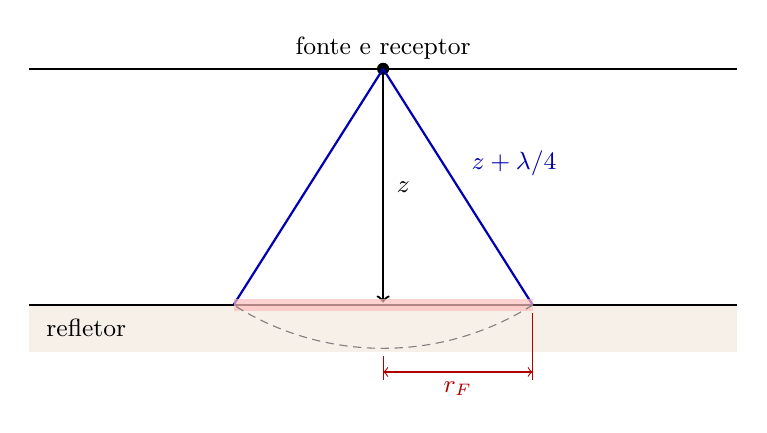
\begin{tikzpicture}[font=\small, x=1cm, y=1cm]
\fill[brown!12] (-4.5,-3.6) rectangle (4.5,-3.0);
\draw[thick] (-4.5,-3.0) -- (4.5,-3.0);
\node[anchor=north west] at (-4.4,-3.05) {refletor};
\draw[thick] (-4.5,0) -- (4.5,0);
\fill (0,0) circle (2.2pt) node[above] {fonte e receptor};
\draw[->, thick] (0,0) -- (0,-2.97);
\node[anchor=west] at (0.05,-1.5) {$z$};
\draw[blue!70!black, thick] (0,0) -- (1.9,-3.0);
\draw[blue!70!black, thick] (0,0) -- (-1.9,-3.0);
\node[anchor=west, blue!70!black] at (1.0,-1.2) {$z + \lambda/4$};
\fill[red!25, opacity=0.7] (-1.9,-3.08) rectangle (1.9,-2.92);
\draw[red!70!black] (0,-3.65) -- (0,-3.95) (1.9,-3.1) -- (1.9,-3.95);
\draw[<->, red!70!black] (0,-3.85) -- (1.9,-3.85) node[midway, below] {$r_F$};
\draw[gray, densely dashed] (-57.6:3.55) arc (-57.6:-122.4:3.55);
\end{tikzpicture}

\par\smallskip{\small A primeira \omterm{def:b3:exploration-seismology:fresnel}{zona de Fresnel} (esquemática): a parte do
refletor cuja distância, a partir de uma fonte e um receptor coincidentes, excede a
distância normal $z$ em menos de $\lambda/4$ (arco tracejado: a esfera de raio
$z + \lambda/4$), de modo que o excesso do percurso de ida e volta fica abaixo de meio comprimento de onda
e suas reflexões chegam em fase. A escala de $\lambda$ está exagerada.}
\label{fig:b3:exploration-seismology:fresnel}
\end{omfigure}

\section{Aquisição e processamento por ponto médio comum}

Um único eco é fraco demais para ser visto no ruído. Por isso, levantamentos de reflexão
registram cada ponto da subsuperfície muitas vezes, com diferentes pares fonte--receptor,
e somam os registros.

\begin{definition}[Ponto médio comum, multiplicidade]\label{def:b3:exploration-seismology:cmp}
Para uma fonte em $x_s$ e um receptor em $x_r$ sobre uma linha, o ponto médio é
$(x_s + x_r)/2$ e o afastamento $x = |x_r - x_s|$. Um agrupamento de \emph{ponto
médio comum}\index{ponto médio comum} (CMP) é o conjunto de traços de todos os
tiros que compartilham o mesmo ponto médio; sobre camadas planas, todos refletem no
mesmo ponto da subsuperfície. A \emph{multiplicidade (de cobertura sísmica)}\index{multiplicidade (de cobertura sísmica)}
é o número de traços em um agrupamento. Com $N$ canais no
intervalo entre receptores $\Delta g$ e um tiro a cada $\Delta s$ ao longo da linha, a
multiplicidade é $N\Delta g/(2\Delta s)$.
\end{definition}

\begin{omfigure}
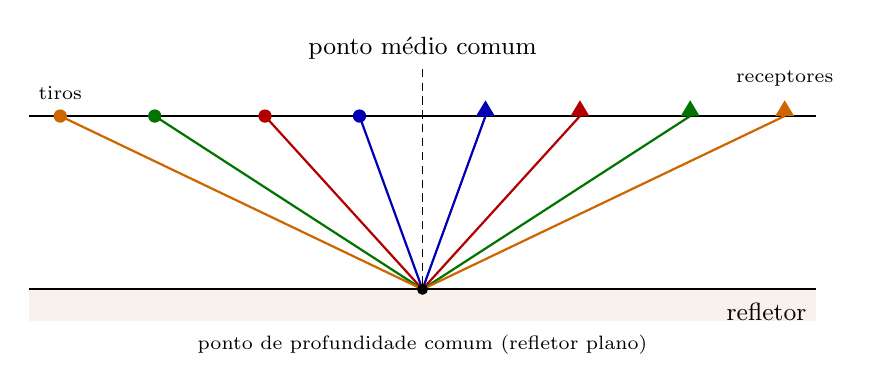
\begin{tikzpicture}[font=\small, x=1cm, y=1cm]
\draw[thick] (-5,0) -- (5,0);
\fill[brown!10] (-5,-2.6) rectangle (5,-2.2);
\draw[thick] (-5,-2.2) -- (5,-2.2);
\node[anchor=north east] at (5,-2.25) {refletor};
\foreach \off/\col in {0.8/blue!70!black, 2.0/red!70!black, 3.4/green!45!black, 4.6/orange!80!black} {
  \draw[\col, thick] (-\off,0) -- (0,-2.2) -- (\off,0);
  \fill[\col] (-\off,0) circle (2.4pt);
  \fill[\col] (\off-0.12,0) -- (\off+0.12,0) -- (\off,0.2) -- cycle;
}
\fill (0,-2.2) circle (2pt);
\draw[densely dashed] (0,0.6) -- (0,-2.2);
\node[anchor=south] at (0,0.6) {ponto médio comum};
\node[anchor=north, align=center, font=\scriptsize] at (0,-2.65) {ponto de profundidade comum (refletor plano)};
\node[anchor=south, font=\scriptsize] at (-4.6,0.08) {tiros};
\node[anchor=south, font=\scriptsize] at (4.6,0.25) {receptores};
\end{tikzpicture}

\par\smallskip{\small Geometria de \omterm{def:b3:exploration-seismology:cmp}{ponto médio comum} (esquemática): quatro pares fonte--receptor
(pontos, triângulos) de afastamentos diferentes compartilham o mesmo ponto médio; sobre um
refletor plano, todos refletem no mesmo ponto abaixo dele. Seus traços formam um
agrupamento de multiplicidade quatro.}
\label{fig:b3:exploration-seismology:cmp}
\end{omfigure}

\begin{theorem}[Sobretempo normal]\label{thm:b3:exploration-seismology:nmo}
Em uma camada de velocidade $v$ sobre um refletor plano, no tempo vertical de ida e volta
$t_0$, a reflexão registrada no afastamento $x$ chega em
\[
  t(x)^2 = t_0^2 + \frac{x^2}{v^2},
\]
uma hipérbole no plano $(x, t)$. O atraso $\Delta t = t(x) - t_0$ é o
\emph{sobretempo normal}\index{sobretempo normal}; para $x \ll vt_0$,
$\Delta t \approx x^2/(2v^2t_0)$.
\end{theorem}

\begin{proof}
O caminho da reflexão vai da fonte até o ponto de reflexão sob o
ponto médio e volta ao receptor: dois trechos de comprimento
$\sqrt{(vt_0/2)^2 + (x/2)^2}$. Assim, $t = (2/v)\sqrt{(vt_0/2)^2 + (x/2)^2}$ e
$t^2 = t_0^2 + x^2/v^2$. Então $t - t_0 = (t^2 - t_0^2)/(t + t_0) \approx
x^2/(2v^2t_0)$.
\end{proof}

Em várias camadas, o tempo de reflexão não é mais exatamente hiperbólico, mas é
praticamente assim para afastamentos pequenos, com uma velocidade que é a média ponderada das
velocidades das camadas.

\begin{definition}[Empilhamento, velocidades média quadrática e intervalar]\label{def:b3:exploration-seismology:velocities}
A \emph{velocidade intervalar}\index{velocidade intervalar} $v_i$ de uma camada é a sua
própria velocidade; com $\Delta t_i = 2h_i/v_i$ o tempo de ida e volta através dela, a
\emph{velocidade média quadrática}\index{velocidade média quadrática} até a
base da camada $n$ é
\[
  V_{\text{rms},n} = \left(\frac{\sum_{i\le n}v_i^2\,\Delta t_i}{\sum_{i\le n}\Delta t_i}\right)^{1/2}.
\]
A \emph{velocidade de empilhamento}\index{velocidade de empilhamento} de uma reflexão é a
velocidade $V$ da hipérbole $t^2 = t_0^2 + x^2/V^2$ que melhor ajusta seus tempos em um
agrupamento CMP.
\end{definition}

\begin{proposition}[Velocidade de empilhamento em afastamentos pequenos]\label{prop:b3:exploration-seismology:rms}
Sobre camadas planas, $t(x)^2 = t_0^2 + x^2/V_{\text{rms}}^2 + O(x^4)$: para
afastamentos pequenos, a \omterm{def:b3:exploration-seismology:velocities}{velocidade de empilhamento} é a \omterm{def:b3:exploration-seismology:velocities}{velocidade média quadrática}.
\end{proposition}

\begin{proof}
Para o \omterm{def:b3:seismology-imaging:ray-parameter}{parâmetro do raio} $p$, $x = \sum_i 2h_i\tan\varphi_i$ e
$t = \sum_i 2h_i/(v_i\cos\varphi_i)$, com $\sin\varphi_i = pv_i$. Até a segunda
ordem em $p$, $\tan\varphi_i \approx pv_i$ e $1/\cos\varphi_i \approx 1 +
p^2v_i^2/2$, logo $x \approx p\sum v_i^2\Delta t_i = pV_{\text{rms}}^2t_0$ e
$t \approx t_0 + \tfrac12p^2V_{\text{rms}}^2t_0$. Então
$t^2 \approx t_0^2 + p^2V_{\text{rms}}^2t_0^2 = t_0^2 + x^2/V_{\text{rms}}^2$, os
termos desprezados sendo de ordem $p^4$, isto é, $x^4$.
\end{proof}

\begin{theorem}[Equação de Dix]\label{thm:b3:exploration-seismology:dix}
Se $V_{n-1}$ e $V_n$ são as \omterm{def:b3:exploration-seismology:velocities}{velocidades médias quadráticas} até o topo e até a base da camada
$n$, nos tempos de ida e volta $t_{n-1}$ e $t_n$, a \omterm{def:b3:exploration-seismology:velocities}{velocidade intervalar} da
camada é dada pela \emph{equação de Dix}\index{equação de Dix}
\[
  v_n^2 = \frac{V_n^2t_n - V_{n-1}^2t_{n-1}}{t_n - t_{n-1}} ,
\]
e sua espessura é $h_n = v_n(t_n - t_{n-1})/2$.
\end{theorem}

\begin{proof}
Por definição, $V_n^2t_n = \sum_{i\le n}v_i^2\Delta t_i$ e $V_{n-1}^2t_{n-1}
= \sum_{i\le n-1}v_i^2\Delta t_i$. A diferença entre elas é $v_n^2\Delta t_n$, com
$\Delta t_n = t_n - t_{n-1}$.
\end{proof}

A análise de velocidades varre cada agrupamento em busca da hipérbole que melhor se ajusta à
energia: para cada par de teste $t_0$ e $V$, os traços são somados ao longo da curva, e
mapeia-se uma medida de coerência (a \textit{semblance}); o analista escolhe seus máximos,
refletor por refletor, para construir uma função de velocidade. A correção de \omterm{thm:b3:exploration-seismology:nmo}{sobretempo normal} então
desloca cada amostra de cada traço de $t(x)$ para $t_0$, achatando as
reflexões, e os traços de cada agrupamento são somados.

\begin{definition}[Empilhamento (sísmico)]\label{def:b3:exploration-seismology:stack}
O \emph{empilhamento (sísmico)}\index{empilhamento (sísmico)} é a soma, após a
correção de \omterm{thm:b3:exploration-seismology:nmo}{sobretempo normal}, dos traços de um agrupamento CMP em um único traço
posicionado no ponto médio. Os traços empilhados, lado a lado ao longo da linha, formam
a seção empilhada, uma imagem dos refletores em tempo de ida e volta.
\end{definition}

\begin{proposition}[Ganho de um empilhamento]\label{prop:b3:exploration-seismology:sqrtN}
Se os $N$ traços de um agrupamento carregam o mesmo sinal de reflexão e ruído independente
de mesmo desvio-padrão $\sigma$, sua média carrega o mesmo sinal
e ruído de desvio-padrão $\sigma/\sqrt N$: o empilhamento eleva a
razão sinal-ruído por $\sqrt N$.
\end{proposition}

\begin{proof}
A variância de uma soma de $N$ variáveis independentes é a soma de suas
variâncias, $N\sigma^2$; dividida por $N^2$, a média tem a variância
$\sigma^2/N$ (o desvio-padrão da média, relembrado dos livros de
matemática).
\end{proof}

\begin{omfigure}
\begin{tikzpicture}
\begin{groupplot}[group style={group size=2 by 1, horizontal sep=0.5cm, y descriptions at=edge left},
  width=0.52\linewidth, height=0.56\linewidth, y dir=reverse, ymin=0.4, ymax=0.92,
  xmin=-150, xmax=2150, tick label style={font=\scriptsize}, title style={font=\small},
  xlabel={\scriptsize deslocamento (\unit{m})}]
\nextgroupplot[title={(a) agrupamento CMP}, ylabel={tempo de ida e volta (\unit{s})}]
\addplot[black, very thin, unbounded coords=jump] table[x=x, y=t] {figdata/out/bachelor-3-cmp_nmo-gather-raw.dat};
\nextgroupplot[title={(b) após a correção de sobretempo normal}]
\addplot[black, very thin, unbounded coords=jump] table[x=x, y=t] {figdata/out/bachelor-3-cmp_nmo-gather-nmo.dat};
\end{groupplot}
\end{tikzpicture}

\par\smallskip{\small Um agrupamento CMP sintético sob o eixo do sinclinal da
linha Varden (calculado por traçado exato de raios através da coluna de camadas planas; \omterm{def:b3:exploration-seismology:wavelet}{ondaleta de Ricker} de 30
Hz; sem ruído). (a) As quatro reflexões (topo do folhelho, topo
e base do calcário, topo do embasamento) curvam-se para baixo com o deslocamento ao longo
de hipérboles aproximadas. (b) Após a correção de \omterm{thm:b3:exploration-seismology:nmo}{sobretempo normal} com as \omterm{def:b3:exploration-seismology:velocities}{velocidades de empilhamento}
ajustadas aos deslocamentos até \qty{600}{m}, as reflexões ficam planas até cerca de
\qty{1}{km}; além disso, os tempos verdadeiros se afastam da hipérbole e a
correção as deixa curvadas, e as ondaletas ficam alongadas; no processamento,
os traços distantes alongados das reflexões rasas são silenciados antes do
empilhamento.}
\label{fig:b3:exploration-seismology:gather}
\end{omfigure}

\begin{omfigure}
\begin{tikzpicture}
\begin{axis}[omrecord, width=0.72\linewidth, height=0.46\linewidth,
  xmin=0.4, xmax=0.78, ymin=2000, ymax=5000,
  xlabel={tempo de ida e volta $t_0$ (\unit{s})}, ylabel={velocidade (\unit{m.s^{-1}})},
  legend cell align=left, legend columns=2,
  legend style={font=\scriptsize, at={(0.5,-0.24)}, anchor=north}]
\addplot[gray, thick, const plot mark right] table[x=t0, y=vint] {figdata/out/bachelor-3-cmp_nmo-vel.dat};
\addlegendentry{velocidade intervalar do modelo}
\addplot[gray, thick, forget plot] coordinates {(0.4,2500) (0.487847,2500)};
\addplot[blue!70!black, thick, mark=*, mark size=1.5pt] table[x=t0, y=vrms] {figdata/out/bachelor-3-cmp_nmo-vel.dat};
\addlegendentry{velocidade média quadrática}
\addplot[red!70!black, only marks, mark=square*, mark size=1.6pt] table[x=t0, y=vstack] {figdata/out/bachelor-3-cmp_nmo-vel.dat};
\addlegendentry{velocidade de empilhamento (deslocamentos até \qty{600}{m})}
\addplot[green!45!black, only marks, mark=triangle*, mark size=2pt] table[x=t0, y=vdix] {figdata/out/bachelor-3-cmp_nmo-vel.dat};
\addlegendentry{velocidade intervalar de Dix}
\end{axis}
\end{tikzpicture}

\par\smallskip{\small Velocidades sob o eixo do sinclinal (calculadas). A \omterm{def:b3:exploration-seismology:velocities}{velocidade
média quadrática}, uma média ponderada, varia lentamente; as \omterm{def:b3:exploration-seismology:velocities}{velocidades de empilhamento} do
agrupamento ficam próximas a ela. Aplicada a elas, a \omterm{thm:b3:exploration-seismology:dix}{equação de Dix} recupera a \omterm{def:b3:exploration-seismology:velocities}{velocidade
intervalar} de cada camada (a linha em degraus, traçada na base de cada camada) com
erro de alguns por cento, sendo o erro maior no calcário fino e rápido.}
\label{fig:b3:exploration-seismology:velocities}
\end{omfigure}

\begin{omfigure}
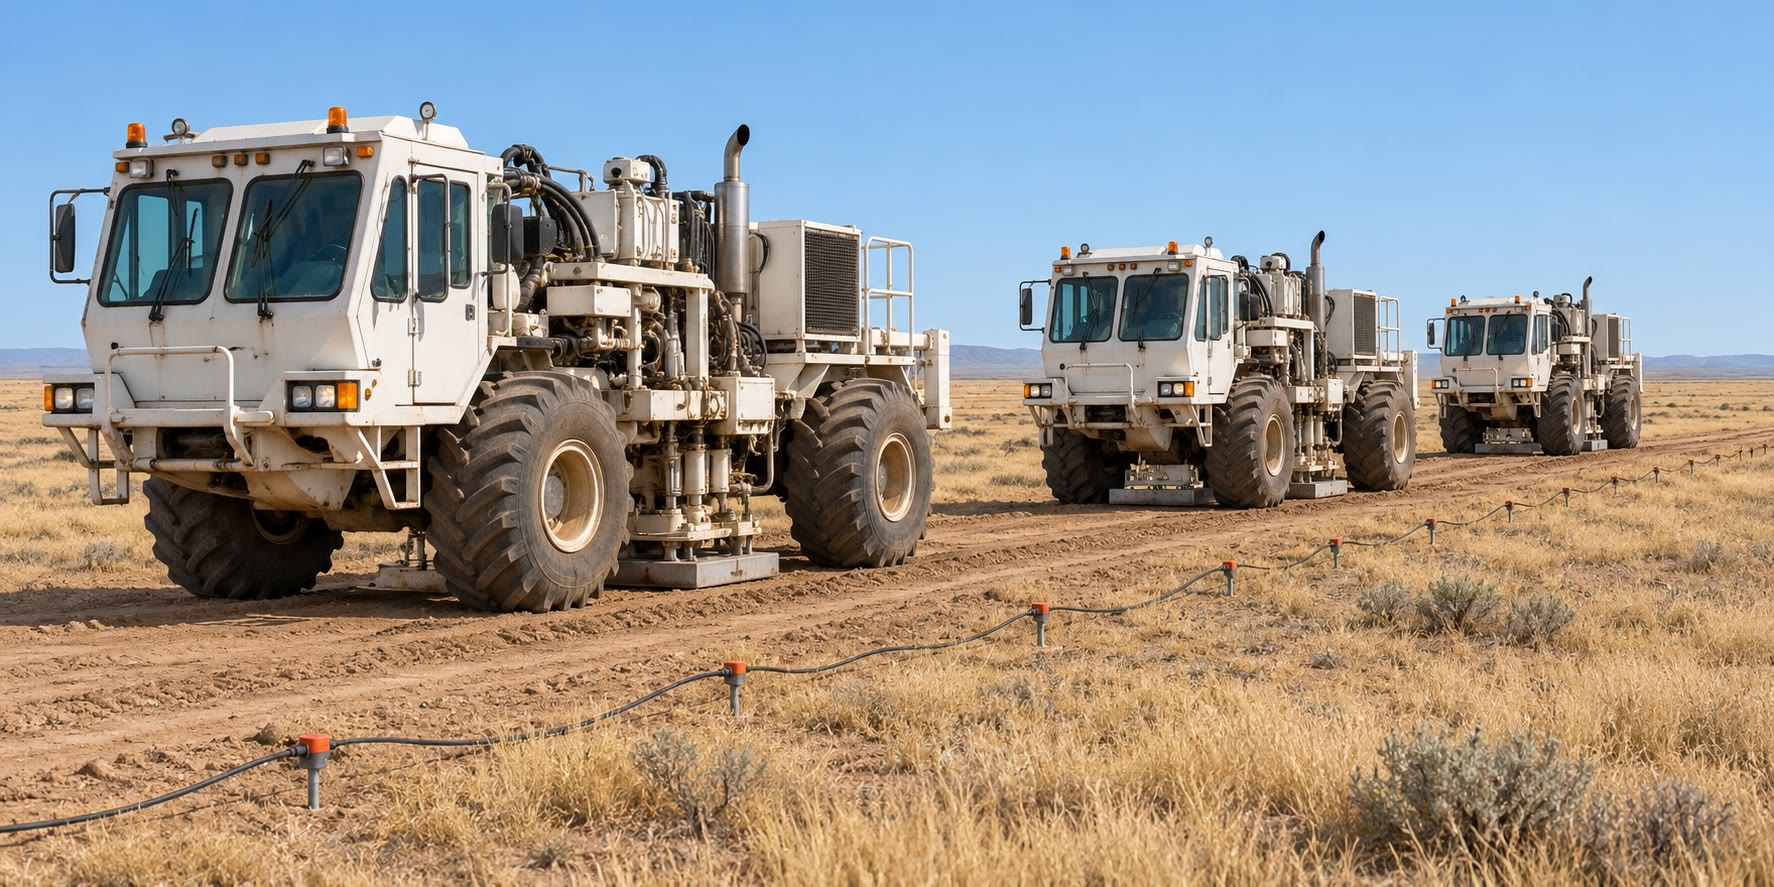
\includegraphics[width=0.62\linewidth]{images/book5/ai/b3-vibroseis.jpg}

\par\smallskip{\small Caminhões vibradores em uma linha de levantamento terrestre: em vez de
uma explosão, cada caminhão pressiona uma placa pesada contra o solo e a faz vibrar com
uma varredura de frequências por vários segundos; os registros longos são comprimidos em
pulsos curtos por correlação com a varredura (Ilustração gerada por IA.)}
\label{fig:b3:exploration-seismology:vibroseis}
\end{omfigure}

\section{Migração}

Uma seção empilhada mostra cada reflexão sob o ponto médio em que foi
registrada, no tempo que levou para voltar. Para um refletor plano, é ali que ela está.
Para um refletor inclinado, não: o eco registrado em um ponto da superfície vem do ponto do
refletor mais próximo a ele, que fica no sentido ascendente do mergulho, e não verticalmente
abaixo. Pontos como os cortes de falha, que espalham energia em todas as
direções, aparecem como hipérboles.

\begin{definition}[Migração sísmica]\label{def:b3:exploration-seismology:migration}
A \emph{migração sísmica}\index{migração sísmica} é a etapa de processamento que
desloca as reflexões de uma seção sísmica para as posições dos refletores que as
produziram: restaura os mergulhos e as posições verdadeiros dos refletores inclinados e
faz colapsar as hipérboles de difração dos espalhadores pontuais sobre seus vértices.
Feita com um modelo de velocidade em tempo, fornece uma seção migrada em tempo; com um
modelo em profundidade, uma imagem em profundidade.
\end{definition}

\begin{theorem}[Mergulho em uma seção de afastamento nulo]\label{thm:b3:exploration-seismology:dip}
Em um meio de velocidade $v$, um refletor plano de mergulho $\theta$ no plano da
seção aparece na seção de afastamento nulo, representada como a profundidade $vt/2$
verticalmente abaixo de cada ponto de registro, como uma linha de mergulho aparente $\theta_a$
com
\[
  \tan\theta_a = \sin\theta .
\]
O refletor registrado no ponto $x$ vem do ponto do refletor a uma distância
$(vt/2)\sin\theta$ no sentido ascendente do mergulho em relação ao ponto verticalmente abaixo de $x$.
\end{theorem}

\begin{proof}
O raio de afastamento nulo é normal ao refletor, logo o tempo registrado em $x$ é
$t = 2d(x)/v$, em que $d(x)$ é a distância de $x$ ao plano. Essa distância
cresce $\sin\theta$ a cada unidade de $x$ na direção do mergulho, de modo que a profundidade
plotada $vt/2 = d(x)$ tem inclinação $\sin\theta$. O pé da normal traçada de $x$
ao plano está a uma distância horizontal $d\sin\theta$ de $x$, do lado ascendente do
mergulho.
\end{proof}

Como $\tan\theta_a = \sin\theta < \tan\theta$, uma seção não migrada sempre mostra
mergulhos mais suaves do que os verdadeiros, e não consegue mostrar mergulhos mais íngremes do que
\ang{45} de forma alguma. Um espalhador pontual à profundidade $z$ abaixo do ponto $x_0$ retorna em
$x$ o tempo de afastamento nulo $t(x) = (2/v)\sqrt{z^2 + (x - x_0)^2}$: uma hipérbole com
seu vértice sobre o ponto, a difração. A migração, em sua forma mais simples,
o empilhamento de difrações, soma cada seção ao longo da hipérbole de difração de
todo espalhador possível e coloca a soma no vértice: os refletores, que são linhas
contínuas de espalhadores, emergem em seus lugares verdadeiros, e as
difrações colapsam.

\begin{omfigure}
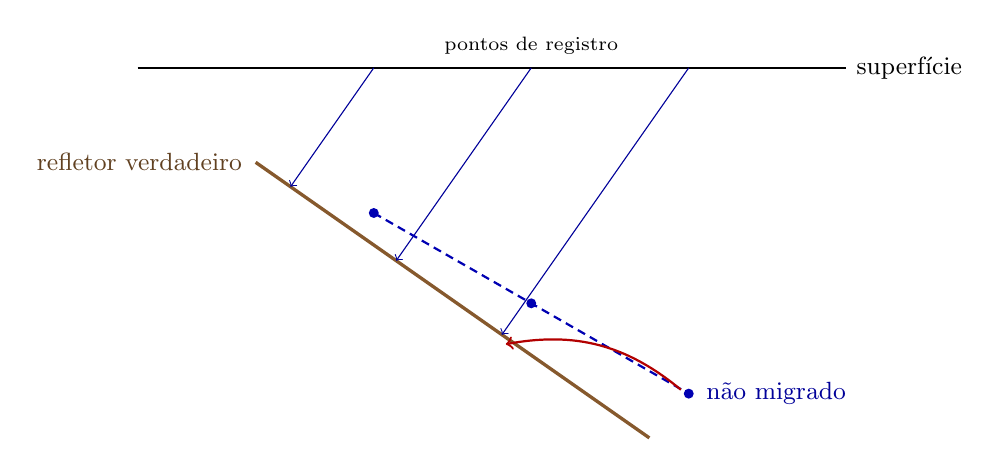
\begin{tikzpicture}[font=\small, x=1cm, y=1cm]
\draw[thick] (-0.5,0) -- (8.5,0) node[right] {superfície};
% true reflector, dip 35 deg, rising to the left
\draw[very thick, brown!70!black] (1.0,-1.2) -- (6.0,-4.70);
\node[brown!50!black, anchor=east] at (0.95,-1.2) {refletor verdadeiro};
% zero-offset normal rays from x = 2, 4, 6
\foreach \x in {2.5, 4.5, 6.5} {
  % distance from (x,0) to the line through (1,-1.2) dir (cos35,-sin35): normal n=(sin35,cos35)
  \pgfmathsetmacro{\dd}{abs(0.5736*(\x-1.0) + 0.8192*(0+1.2))}
  \draw[blue!60!black, ->] (\x,0) -- ++({-0.5736*\dd},{-0.8192*\dd});
  \fill[blue!70!black] (\x,{-\dd}) circle (1.8pt);
}
% apparent reflector through the plotted points
\pgfmathsetmacro{\da}{abs(0.5736*1.5 + 0.8192*1.2)}
\pgfmathsetmacro{\db}{abs(0.5736*5.5 + 0.8192*1.2)}
\draw[blue!70!black, thick, densely dashed] (2.5,{-\da}) -- (6.5,{-\db});
\node[blue!60!black, anchor=west] at (6.6,{-\db}) {não migrado};
\node[anchor=south, font=\scriptsize] at (4.5,0.05) {pontos de registro};
\draw[->, red!70!black, thick] (6.4,{-\db+0.05}) to[bend right=25] ({6.5-0.5736*\db+0.05},{-0.8192*\db-0.12});
\end{tikzpicture}

\par\smallskip{\small Migração de um refletor inclinado (esquemático, mergulho
verdadeiro \ang{35}). O raio de afastamento nulo em cada ponto de registro é
normal ao refletor, de modo que seu eco vem do lado de cima do mergulho; plotado
verticalmente abaixo do ponto, à profundidade $vt/2$, a reflexão aparece mais suave (tracejado: $\tan\theta_a =
\sin\theta$, aqui \ang{29.8}), e deslocada no sentido do mergulho. A migração (seta vermelha) a desloca de volta.}
\label{fig:b3:exploration-seismology:migration}
\end{omfigure}

\section{Estratigrafia sísmica}

Uma seção migrada é um retrato do acamamento, e pode ser lida como
estratigrafia: as reflexões seguem as superfícies de acamamento, que são
linhas de tempo, de modo que sua geometria registra como a bacia foi preenchida.

\begin{definition}[Estratigrafia sísmica, fácies sísmica]\label{def:b3:exploration-seismology:seismic-stratigraphy}
A \emph{estratigrafia sísmica}\index{estratigrafia sísmica} é a interpretação
da estratigrafia e da história deposicional de uma bacia a partir da geometria
de suas reflexões sísmicas. Uma \emph{fácies sísmica}\index{fácies sísmica} é uma
unidade tridimensional de reflexões cujo caráter (continuidade, amplitude,
frequência, geometria interna: paralela, divergente, sigmoidal, caótica, em montes)
difere daquele de suas vizinhas e é interpretada como um
ambiente de deposição.
\end{definition}

\begin{definition}[Terminações de refletores]\label{def:b3:exploration-seismology:terminations}
Uma \emph{terminação de refletor}\index{terminação de refletor} é o fim de uma
reflexão contra outra. \emph{Onlap}\index{onlap}: uma reflexão inicialmente
horizontal termina contra uma superfície que sobe com maior inclinação, os
estratos mais jovens se apoiando sobre uma encosta mais antiga. \emph{Downlap}\index{downlap}: uma reflexão inclinada
termina, no sentido do mergulho, contra uma superfície mais suave, como as
bases frontais de estratos progradantes repousam sobre o assoalho de uma bacia. \emph{Toplap}\index{toplap}: reflexões inclinadas
terminam, no sentido contrário ao do mergulho, contra uma superfície sobreposta, com pouca erosão, como
os topos de estratos progradantes encontram o nível do mar. \emph{Truncamento
erosivo}\index{truncamento erosivo}: reflexões terminam, no sentido contrário ao do mergulho, contra uma
superfície sobreposta que as corta, uma discordância.
\end{definition}

\begin{omfigure}
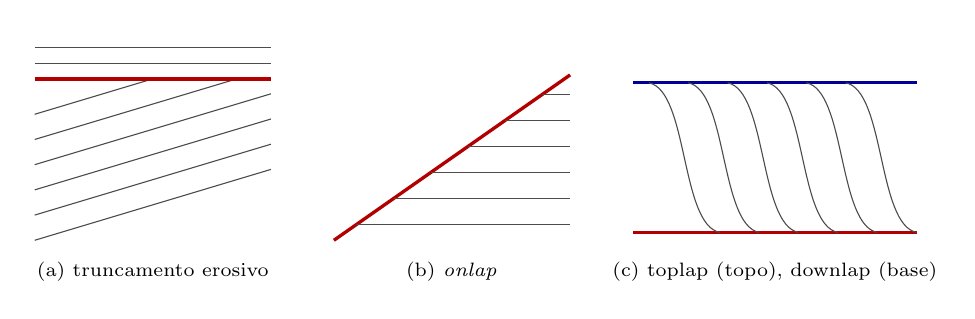
\begin{tikzpicture}[font=\scriptsize, x=1cm, y=1cm]
% erosional truncation: tilted beds cut by an unconformity
\begin{scope}
\foreach \k in {0,...,5} {\draw[gray!60!black] (0,{-2.3+0.32*\k}) -- (3.0,{-1.4+0.32*\k-0.25*0});}
\fill[white] (0,-0.25) -- (3.2,-0.25) -- (3.2,0.4) -- (0,0.4) -- cycle;
\draw[very thick, red!70!black] (0,-0.25) -- (3.0,-0.25);
\foreach \k in {0,1} {\draw[gray!60!black] (0,{-0.05+0.2*\k}) -- (3.0,{-0.05+0.2*\k});}
\node[anchor=north] at (1.5,-2.45) {(a) truncamento erosivo};
\end{scope}
% onlap
\begin{scope}[xshift=3.8cm]
\draw[very thick, red!70!black] (0,-2.3) -- (3.0,-0.2);
\foreach \k in {0,...,5} {\pgfmathsetmacro{\y}{-2.1+0.33*\k} \pgfmathsetmacro{\xe}{(\y+2.3)/0.7} \draw[gray!60!black] (\xe,\y) -- (3.0,\y);}
\node[anchor=north] at (1.5,-2.45) {(b) \textit{onlap}};
\end{scope}
% downlap and toplap: clinoforms
\begin{scope}[xshift=7.6cm]
\draw[very thick, red!70!black] (0,-2.2) -- (3.6,-2.2);
\draw[very thick, blue!60!black] (0,-0.3) -- (3.6,-0.3);
\foreach \k in {0,...,5} {\draw[gray!60!black] ({0.2+0.5*\k},-0.3) .. controls ({0.7+0.5*\k},-0.4) and ({0.6+0.5*\k},-2.1) .. ({1.1+0.5*\k},-2.2);}
\node[anchor=north] at (1.8,-2.45) {(c) toplap (topo), downlap (base)};
\end{scope}
\end{tikzpicture}

\par\smallskip{\small Terminações de refletores (seções esquemáticas, reflexões em
cinza, superfícies terminais em cor). (a) Reflexões inclinadas cortadas por uma
discordância. (b) Reflexões horizontais terminando contra uma encosta mais antiga. (c) Estratos inclinados
de uma cunha progradante terminando, no sentido contrário ao do mergulho, contra a superfície acima (\omterm{def:b3:exploration-seismology:terminations}{toplap}) e
no sentido do mergulho, sobre o assoalho da bacia (\omterm{def:b3:exploration-seismology:terminations}{downlap}).}
\label{fig:b3:exploration-seismology:terminations}
\end{omfigure}

As terminações marcam as superfícies que delimitam sequências de camadas
geneticamente relacionadas; mapeá-las em uma bacia e relacioná-las à subida e
descida do nível relativo do mar é a estratigrafia de sequências, assunto do
\cref{ch:b3:sequence-stratigraphy}. Uma seção sísmica de uma margem passiva
costuma mostrar cunhas de reflexões progradantes em direção ao mar que fazem \omterm{def:b3:exploration-seismology:terminations}{downlap}
sobre o assoalho profundo, coroadas por \omterm{def:b3:exploration-seismology:terminations}{toplap}, e enterradas, no sentido
do continente, sob estratos em \omterm{def:b3:exploration-seismology:terminations}{onlap} depositados quando o mar voltou a subir.

\begin{inthefield}[Um levantamento marinho com streamers e uma equipe em terra]
\begin{minipage}[t]{0.55\linewidth}\vspace{0pt}
Em um levantamento marinho o navio nunca para: ele navega linha após linha a
poucos nós, os arranjos de canhões de ar disparando em intervalos fixos, os streamers mantidos a
profundidade constante por pequenas asas direcionáveis e localizados por acústica e satélite
posicionamento. Observadores na ponte acompanham o mar ao redor do arranjo, e o
levantamento segue regras que estabelecem as medidas de proteção aos mamíferos marinhos,
a vigilância mantida e o que deve ser relatado.
% ledger: noaa5:itr-gom
Em terra a equipe dispõe cabos ou unidades de registro sem fio ao longo das linhas;
caminhões vibradores avançam em comboio de um ponto de fonte ao seguinte, e um
caminhão de registro verifica cada canal antes de cada varredura. De volta ao
centro de processamento, os registros são ordenados em famílias de \omterm{def:b3:exploration-seismology:cmp}{ponto médio comum}, as
velocidades são escolhidas, os dados são empilhados e migrados, e a seção é entregue aos
intérpretes.
\end{minipage}\hfill
\begin{minipage}[t]{0.42\linewidth}\vspace{0pt}
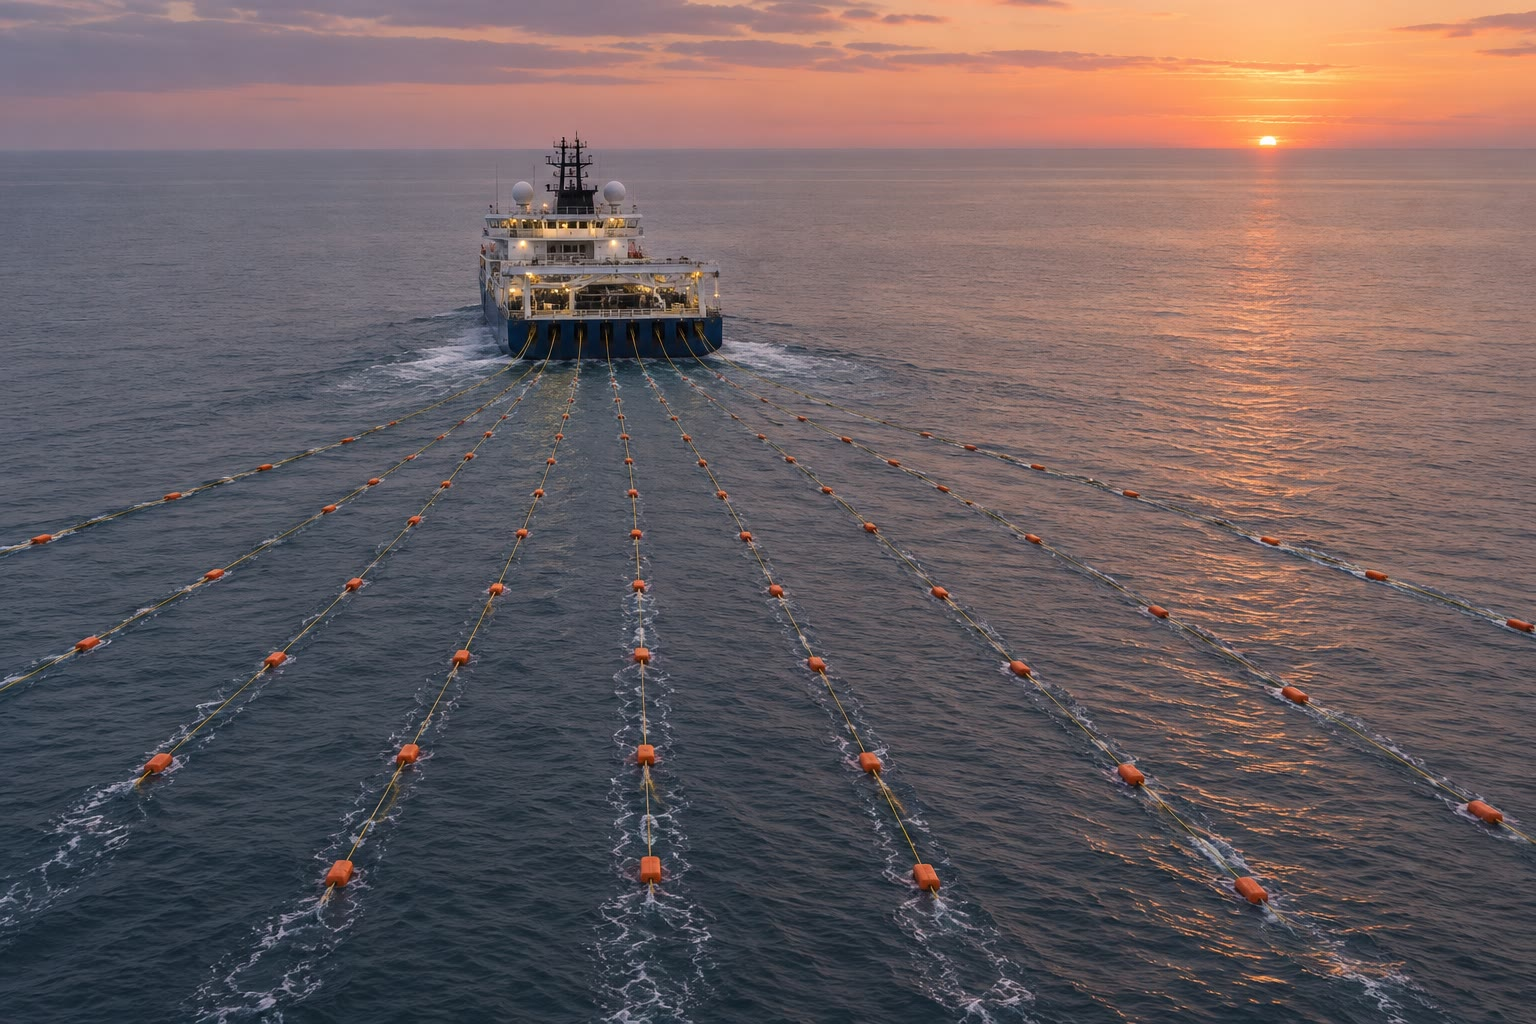
\includegraphics[width=\linewidth]{images/book5/ai/b3-streamer-vessel.jpg}

{\scriptsize Um navio de levantamento sísmico rebocando seus streamers ao entardecer
(Ilustração gerada por IA).}
\end{minipage}
\end{inthefield}

\section{Exercícios}

\begin{exercise}[$\star$]\label{exo:b3:exploration-seismology:1}
Giz ($v = \qty{2500}{m.s^{-1}}$, $\rho = \qty{2.00}{g.cm^{-3}}$) repousa sobre folhelho
(\qty{2300}{m.s^{-1}}, \qty{2.30}{g.cm^{-3}}), que repousa sobre calcário
(\qty{4500}{m.s^{-1}}, \qty{2.60}{g.cm^{-3}}). Calcule as três impedâncias e
os coeficientes de reflexão das duas interfaces. Que fração da energia incidente
a parte superior do calcário reflete?
% ledger: mavko:velocities
\end{exercise}

\begin{exercise}[$\star$]\label{exo:b3:exploration-seismology:2}
Um refletor plano jaz a \qty{800}{m} abaixo de uma camada com velocidade de \qty{2000}{m.s^{-1}}.
Calcule $t_0$, o tempo de reflexão a um afastamento de \qty{1000}{m}, e o \omterm{thm:b3:exploration-seismology:nmo}{sobretempo normal}
nesse ponto. Compare com a aproximação $x^2/(2v^2t_0)$.
\end{exercise}

\begin{exercise}[$\star$]\label{exo:b3:exploration-seismology:3}
Um streamer tem 240 canais espaçados de \qty{12.5}{m}, e o navio dispara a cada
\qty{25}{m}. Calcule o intervalo entre pontos médios comuns e a multiplicidade. Qual intervalo entre tiros
resultaria em uma multiplicidade de 120?
\end{exercise}

\begin{exercise}[$\star$]\label{exo:b3:exploration-seismology:4}
Com frequência dominante de \qty{30}{Hz}, calcule o comprimento de onda e o
quarto do comprimento de onda no arenito de \qty{3000}{m.s^{-1}} e no calcário de
\qty{4500}{m.s^{-1}}. Calcule o raio da primeira \omterm{def:b3:exploration-seismology:fresnel}{zona de Fresnel} de um
refletor a \qty{1000}{m} de profundidade sob rochas de velocidade média de \qty{2800}{m.s^{-1}}.
\end{exercise}

\begin{exercise}[$\star\star$]\label{exo:b3:exploration-seismology:5}
Duas reflexões têm $t_0 = \qty{0.500}{s}$ com \omterm{def:b3:exploration-seismology:velocities}{velocidade média quadrática} de
\qty{2400}{m.s^{-1}}, e $t_0 = \qty{0.700}{s}$ com \qty{2800}{m.s^{-1}}.
Calcule a \omterm{def:b3:exploration-seismology:velocities}{velocidade intervalar} e a espessura da camada entre elas.
\end{exercise}

\begin{exercise}[$\star\star$]\label{exo:b3:exploration-seismology:6}
Um refletor plano tem mergulho $\varphi$ no plano de uma linha de \omterm{def:b3:exploration-seismology:cmp}{ponto médio comum}, em uma camada de
velocidade $v$. (a) Mostre que $t(x)^2 = t_0^2 + x^2\cos^2\varphi/v^2$, em que $t_0$ é
o tempo de afastamento nulo no ponto médio. (Dica: use a imagem do ponto médio no
refletor.) (b) Deduza a \omterm{def:b3:exploration-seismology:velocities}{velocidade de empilhamento} e calcule-a para
$v = \qty{2000}{m.s^{-1}}$ e $\varphi = \ang{12}$.
\end{exercise}

\begin{exercise}[$\star\star$]\label{exo:b3:exploration-seismology:7}
Uma família de traços de multiplicidade 60 tem ruído independente, de mesma variância, em cada traço. Por
que fator o empilhamento eleva a razão sinal-ruído? Por que fator a multiplicidade deve ser aumentada
para dobrá-la novamente?
\end{exercise}

\begin{exercise}[$\star\star$]\label{exo:b3:exploration-seismology:8}
Em uma seção de tempo de afastamento nulo, em rocha de \qty{3000}{m.s^{-1}}, uma reflexão
sobe \qty{0.40}{s} de tempo duplo por quilômetro ao longo da linha. Converta essa
inclinação em mergulho aparente, e calcule o mergulho verdadeiro do refletor.
\end{exercise}

\begin{exercise}[$\star\star$]\label{exo:b3:exploration-seismology:9}
Calcule a convolução da \omterm{def:b3:exploration-seismology:synthetic}{série de refletividade} $r = (0, 0.3, 0, -0.2, 0)$ com a
ondaleta de três amostras $w = (-0.5, 1, -0.5)$, amostra por amostra. Onde estão as duas
reflexões? Elas se sobrepõem?
\end{exercise}

\begin{exercise}[$\star\star\star$]\label{exo:b3:exploration-seismology:10}
Um perfil de refração invertido sobre uma camada de \qty{1800}{m.s^{-1}} fornece uma
velocidade aparente no sentido do mergulho de \qty{2900}{m.s^{-1}} e uma no sentido contrário ao mergulho de
\qty{4400}{m.s^{-1}}. Calcule o ângulo crítico, o mergulho e a
velocidade do refrator. Compare a velocidade do refrator com a média harmônica das duas
velocidades aparentes.
\end{exercise}

\begin{exercise}[$\star\star\star$]\label{exo:b3:exploration-seismology:11}
Na \cref{prop:b3:exploration-seismology:tuning}, a camada tem coeficientes de reflexão
$+R$ e $-R$. (a) Mostre que, para $\Delta t \ll T$, o sinal composto
é aproximadamente $R\,\Delta t\,w'(t)$, a derivada no tempo da ondaleta
multiplicada pela espessura da camada em tempo duplo. (b) Explique por que uma camada delgada ainda pode ser
detectada, embora não resolvida, e como sua espessura poderia ser estimada a partir de
sua amplitude. (c) Duas camadas da mesma rocha, com 5 e \qty{10}{m} de espessura, são
imageadas com a mesma ondaleta: qual é a razão entre suas amplitudes?
\end{exercise}

\begin{exercise}[$\star\star\star$]\label{exo:b3:exploration-seismology:12}
Um espalhador pontual jaz a \qty{600}{m} abaixo da linha, em rocha de
\qty{3000}{m.s^{-1}}. (a) Escreva o tempo de afastamento nulo de sua difração em função
da distância horizontal $x$ até o ponto da superfície situado acima dele, e calcule-o em $x = 0$
e em \qty{300}{m}. (b) Mostre que a difração é uma hipérbole com a forma do \omterm{thm:b3:exploration-seismology:nmo}{sobretempo normal}
com velocidade $v/2$, e explique por que uma difração é sempre mais encurvada que uma
reflexão com o mesmo tempo no ápice. (c) O que a migração faz com ela?
\end{exercise}

\section{Problema: uma linha sísmica sobre as Varden Hills}

\begin{problem}[{Problema de fim de semana --- refração, análise de velocidades, profundidade
conversão em profundidade e migração ao longo da seção A--B de Varden Hills}]
\label{pb:b3:exploration-seismology:1}
% values: calc/ch02.py, from figdata seismic_model.py, refraction_dip.py, cmp_nmo.py
Uma linha sísmica é adquirida ao longo da seção A--B de Varden Hills, a região dos
mapas geológicos dos volumes anteriores. Suas distâncias $s$ são contadas a partir de
A ao longo da linha. A cobertura, do topo para a base, é giz, folhelho (\qty{100}{m}),
calcário (\qty{180}{m}) e arenito (\qty{120}{m}), repousando em discordância sobre
um embasamento de xisto; ela é dobrada em um anticlinal e um sinclinal e cortada por uma
falha normal.

\medskip
\noindent\textbf{Parte I --- Um arranjo de refração no flanco oeste.} Um arranjo de
\qty{1200}{m} é disposto entre os pontos de tiro O ($s = \qty{300}{m}$) e L
($s = \qty{1500}{m}$), em terreno tomado como plano. O giz e o folhelho acima do
calcário são tratados como uma única camada de $v_1 = \qty{2.40}{km.s^{-1}}$. Os
tempos da onda de cabeça lidos nos registros são, de O para L, \qty{425.2}{ms} a
\qty{800}{m} e \qty{486.1}{ms} a \qty{1200}{m}; de L para O,
\qty{372.4}{ms} a \qty{800}{m} e \qty{486.1}{ms} a \qty{1200}{m}.
\begin{enumerate}
  \item Calcule as duas velocidades aparentes. Qual dos tiros fica no sentido contrário ao mergulho?
  \item Calcule o ângulo crítico e o mergulho do refrator.
  \item Calcule a velocidade do refrator. Qual é essa rocha?
  \item Calcule os tempos de interceptação e as profundidades perpendiculares do
        refrator sob O e sob L.
  \item Converta-as em profundidades verticais e verifique o mergulho a partir das duas profundidades.
  \item O folhelho sob o giz é mais lento que o giz. O que o levantamento de
        refração faz dele, e como isso enviesa as profundidades?
\end{enumerate}

\noindent\textbf{Parte II --- Análise de velocidade no ponto médio comum S.} Mais a leste, o \omterm{def:b3:exploration-seismology:cmp}{ponto médio comum} S
está sobre o eixo do sinclinal, no bloco abatido da falha, onde
as camadas são tomadas como horizontais. Quatro reflexões são escolhidas no afastamento zero e em
\qty{600}{m}:
\begin{center}
\small
\begin{tabular}{lcccc}
\hline
reflexão & 1 & 2 & 3 & 4 \\
$t_0$ (\unit{s}) & 0.4878 & 0.5748 & 0.6548 & 0.7348 \\
$t(\qty{600}{m})$ (\unit{s}) & 0.5437 & 0.6240 & 0.6887 & 0.7648 \\
\hline
\end{tabular}
\end{center}
\begin{enumerate}[resume]
  \item Calcule a velocidade de \omterm{thm:b3:exploration-seismology:nmo}{sobretempo normal} $V = x/\sqrt{t^2 - t_0^2}$ das reflexões 1
        e 2. Por que a segunda é menor que a primeira?
  \item Calcule-a para as reflexões 3 e 4.
  \item Tomando-as como \omterm{def:b3:exploration-seismology:velocities}{velocidades médias quadráticas}, calcule a \omterm{def:b3:exploration-seismology:velocities}{velocidade intervalar} de cada
        camada pela \omterm{thm:b3:exploration-seismology:dix}{equação de Dix}.
  \item Identifique as camadas pelas suas velocidades, e dê nome às quatro
        interfaces refletoras.
  \item A reflexão 1 é a mais fraca nos registros. Por quê?
  \item Por que as velocidades foram medidas apenas nos afastamentos até \qty{600}{m}
        apenas, quando o arranjo alcança \qty{2}{km}?
\end{enumerate}

\noindent\textbf{Parte III --- Conversão em profundidade e resolução.}
\begin{enumerate}[resume]
  \item Calcule o tempo de ida e volta gasto em cada camada e a sua espessura.
  \item Calcule a profundidade de cada interface refletora abaixo do solo. Compare
        as espessuras do folhelho, do calcário e do arenito com os valores
        dados acima.
  \item Calcule a velocidade média desde o solo até o embasamento, e explique por que
        a velocidade de \omterm{thm:b3:exploration-seismology:nmo}{sobretempo normal} da reflexão 4 superestimaria a profundidade se fosse usada
        no lugar.
  \item A ondaleta do levantamento tem pico em \qty{30}{Hz}. Calcule o comprimento de onda no
        folhelho e a sua \omterm{def:b3:exploration-seismology:resolution}{espessura de sintonia}, tanto pela regra do quarto de comprimento de onda
        e por $b = v/(5.2f)$ para uma \omterm{def:b3:exploration-seismology:wavelet}{ondaleta de Ricker}. O folhelho é resolvido? Em
        que frequência ele entraria em sintonia pela regra do quarto de comprimento de onda?
  \item Calcule o raio da primeira \omterm{def:b3:exploration-seismology:fresnel}{zona de Fresnel} no embasamento, tomando
        $\lambda$ a partir da velocidade de \omterm{thm:b3:exploration-seismology:nmo}{sobretempo normal} da reflexão 4.
\end{enumerate}

\noindent\textbf{Parte IV --- Migração e a falha.}
\begin{enumerate}[resume]
  \item Próximo à falha, o corte do calcário produz uma difração
        cujo vértice está em \qty{0.550}{s}; a \qty{200}{m} do vértice ao longo da linha
        ela está em \qty{0.5732}{s}. Escreva o tempo de difração no afastamento zero e
        deduza a velocidade média acima do corte.
  \item Calcule a profundidade do corte abaixo do solo.
  \item No flanco leste, a reflexão do topo do calcário na seção empilhada
        sobe em direção ao anticlinal, \qty{0.167}{s} de tempo de ida e volta por
        quilômetro, sob rochas de velocidade média \qty{2.48}{km.s^{-1}}. Calcule seu
        mergulho aparente e o seu mergulho verdadeiro.
  \item Uma reflexão nesse flanco é registrada em $t = \qty{0.655}{s}$. Até onde,
        e em que sentido, a migração a desloca?
  \item Através da falha, a reflexão do topo do embasamento sofre um salto de \qty{0.160}{s};
        o bloco abatido carrega a espessura extra no giz. Calcule o
        rejeito.
  \item Dê a profundidade da discordância do embasamento abaixo do \omterm{def:b3:exploration-seismology:cmp}{ponto médio comum} S, a partir das
        \omterm{def:b3:exploration-seismology:velocities}{velocidades intervalares} da Parte II.
\end{enumerate}
\end{problem}
